%
% Manchester Raspberry Jam Workshop Booklet
%
% This template is designed to try and aide consistency between each booklet.
% Insert files as instructed by comments, things like tables of contents are created by other linked files
%

% Is this document PRINT or WEB format?
% (you can use the toggle to cut content for paper, see etoolbox)
\newif\ifprint
\printfalse

% Page Formatting
\ifprint
	\documentclass[a4paper, twocolumn, twoside, 11pt]{article}
	\usepackage[margin=2cm]{geometry}
	\setlength{\columnsep}{1.25cm}
	\setlength{\parskip}{6pt}
\else
	\documentclass[a4paper, onecolumn, oneside, 11pt]{article}
	\usepackage[margin=3cm]{geometry}
	\setlength{\parskip}{9pt}
\fi



% FONT and text format
\usepackage[utf8x]{inputenc}	
\usepackage[UKenglish]{babel}
\ifprint
	\usepackage[usenames, dvipsnames]{color}				%Font Colour
	\usepackage[colorlinks=false]{hyperref}	%URLs
\else
	\usepackage[T1]{fontenc}
	\usepackage[sfdefault]{roboto}
	\usepackage[T1]{fontenc}
	\usepackage[usenames, dvipsnames]{color}				%Font Colour
	\usepackage[colorlinks=true,linkcolor=black,urlcolor=WildStrawberry]{hyperref}
\fi



% Table of Contents Format
\usepackage{tocloft}
\addtocontents{toc}{\cftpagenumbersoff{subsection}}
\setcounter{tocdepth}{2}
\setcounter{secnumdepth}{2}



% Section spacing
\ifprint
	\usepackage[compact]{titlesec}
\fi



% Listings and Asides
\usepackage{McrRaspJam/common/listings}
\usepackage{McrRaspJam/common/asides}



%Clear page for web version
\newcommand{\webclearpage}{
	\ifprint
	\else
		\clearpage
	\fi
}

% misc.
\usepackage{enumitem}									%List spacing changes
\usepackage[toc,page]{appendix}							%Appendix package
\usepackage{graphicx}									% TOC?
\usepackage{etoolbox}									%Boolean used for print/web switching
\usepackage{fancyvrb}									%Centered verbatim

% Enter the document title here
\newcommand{\workshopTitle}{Workshop 14a: Python}

% Enter the author of this workshop
\newcommand{\workshopAuthor}{Written by 
\includegraphics[height=10pt]{McrRaspJam/014_Python/creative-pi-1024}}


\begin{document}
	% Title Format
\ifprint
	\title{Manchester Raspberry Jam \\ \workshopTitle}
	\author{}
\else
	\title{
		\begin{center}
			
\includegraphics[width=30mm]{McrRaspJam/common/logo-512}
		\end{center}
		\vspace{12pt}
		\workshopTitle
	}
	\author{
		Written by \workshopAuthor
	}
\fi

\date{\vspace{-16pt}}
\maketitle


% Online download location
\ifprint
	\begin{mdframed}[rightline=false, leftline=false]
		\scriptsize
		This booklet is available online at \mbox{\href{https://drive.google.com/open?id=0B_1SFjX_5JrmfnhpX0pPRXl6bmJNal8zdUxMeWZOdjJyZVdzU3V6UnBGdlVIMENtbFFkbVk}{bit.ly/McrRaspJam}}
		\normalsize
	\end{mdframed}
\fi

	%Place a SINGLE paragraph summary here
	This workshop focuses on the basics of Python and using it with the Sense HAT.

	%Difficulty
	\textit{Difficulty: Introductory workshop}

	\ifprint
		\renewcommand{\baselinestretch}{0.75}\normalsize
		\tableofcontents
		\renewcommand{\baselinestretch}{1.0}\normalsize
	\else
		\tableofcontents
	\fi

	%
	% Input the main CONTENT below, sans title page or contents.
	% Recommend inputting per section, and adding page breaks here.
	%
	% \webclearpage command is provided, will break page for web format only.
	%

	\setcounter{section}{-1}
\section{Introduction}

	Python is a computer programming language designed for general-purpose use and can be found in use almost everywhere. Python was designed to be easy to read and write, making it the perfect language to start off with!

	Python has been around since 1991 and grew to be popular in 2003, where it was ranked in the top ten most popular programming languages (and it's still there!). It was the programming language of the year in 2007 and 2010 and even comes pre-installed on your Pi!

	%Difficulty
	This is an introductory workshop. Once you're familiar with using your Pi on the desktop, you should be ready to attempt this workshop.

	\subsection*{How to use these booklets}

		The aim of these booklets is to help you attempt these workshops at home, and to explain concepts in more detail than at the workshop. You don't need to refer to use these booklets during the workshop, but you can if you'd like to.

		%Code Listings
		\subsection*{Code listings \& asides}
	
	When you need to make changes to your code, they'll be presented in boxes like the following:

	\lstinputlisting[style=Python]{McrRaspJam/011_Motors/0_introduction/helloworld.py}
	
	You might not need to copy everything, so check the line numbers to make sure you're not copying something twice.
		Occasionally, something will be explained in greater detail in asides, like the one below. You can read these as you wish.
	
\begin{aside}
	Red lines beginning with number signs (\#) are called \textbf{comments}.
	They are ignored by the program, so we can use them to label pieces of code.
\end{aside}

		%All of our workshop resources are available to download from a Google Drive at
\url{http://bit.ly/mcrraspjam}.
There, you can find a PDF copy of this booklet, as well as template and completed program files for each workshop.

	\subsection*{What you'll need}

		For this workshop, you'll just need a working Raspberry Pi running a Linux operating system like Raspbian with Python installed. Luckily for us, Raspbian (and many other Linux distributions) include Python right out of the box.

	\subsection*{Everything else}

		%Aknowledgements
		\ifprint\else These booklets were created using \textrm{\LaTeX}, an advanced typesetting system used for several sorts of books, academic reports and letters. \fi

		%License spiel
		To allow modification and redistribution of these booklets, they are distributed under the \hbox{CC BY-SA 4.0} License.
		Latex source documents are available at \url{http://github.com/McrRaspJam/booklet-workshops}

		\clearpage

	\section{IDLE}

	IDLE is Python's editor, used to edit and run Python programs on your Pi. You can find it under \texttt{Programming > IDLE} from the Raspberry Pi logo in the top left of your screen. There may be more than 1 version of IDLE, as Raspbian comes with both Python 2 and Python 3 installed. Python 3 is the preferred choice (although this booklet will work with Python 2 as well), as it has some improvements over Python 2.

	IDLE opens into it's shell by default, allowing you to enter code and have it run immediately without having to create and save any files. Note that this shell doesn't save your code for you, so make sure you save any code you want to keep!

	\ifprint
	\else
		\begin{center}
			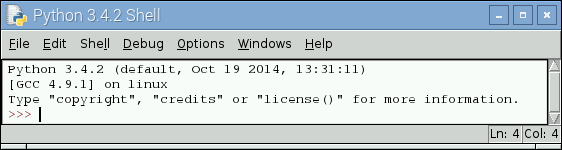
\includegraphics[width=120mm]{McrRaspJam/014_Python/1_idle/screenshot}
		\end{center}
	\fi

	Try typing the following code into the shell and hitting enter.

	\lstinputlisting[style=Python, numbers=none]{McrRaspJam/014_Python/1_idle/hello_world.py}

	You should get the following output after hitting enter.

	\begin{lstlisting}[style=Terminal, numbers=none]
Hello, World!
	\end{lstlisting}

	Now, compare that to the equivalent Java program:

	\lstinputlisting[style=Java, numbers=none, breaklines=true]{McrRaspJam/014_Python/1_idle/HelloWorld.java}

	As opposed to Java, Python is a simple language in which a lot of functionality is implicit and not explicit. There is no need for \texttt{System.out.println} or even the \texttt{main} function, as Python provides them for you.

	\begin{aside}[Execution]
		Code in Python is executed from top to bottom in every file, meaning no \texttt{main} method is required. Simply placing the code in a file is enough for it to run!
	\end{aside}

		\webclearpage

	\section{The Basics}
	\subsection{Variables}

		Variables in Python are just names for a value, like a label on a box. Variables can contain any type, and their type and contents can even change throughout the program's execution!

		You can declare a variable by simply giving it a name and a value as shown below.

		\lstinputlisting[style=Python, numbers=none]{McrRaspJam/014_Python/2_basics/variables.py}

		In this code we create a variable called \texttt{name} containing a person's name and print the variable's contents.

		\textbf{Extra:} Why not try changing this to say your name?

	\subsection{Loops}

		Loops in programming allow us to run some code multiple times, meaning we don't have to repeat ourselves if we want something doing more than once. There are two types of loops in Python called \texttt{for} and \texttt{while} loops.

		The \texttt{for} loop allows us to run some code a specific number of times, an example being printing the numbers 1 through 10.

	  \lstinputlisting[style=Python, numbers=none]{McrRaspJam/014_Python/2_basics/loops.py}

		The above \texttt{for} loop runs through a list of numbers from 1 to 10 in order, which is what the \texttt{range} function has provided us with.

		\textbf{Extra:} Why not try modifying this code to print your name 10 times?

	\subsection{Conditional Statements}

		\textbf{Conditional statements} are used to selectively run code based on a condition. This can be useful as we can only run specific code when we want to. In this example we'll change our code so that it only prints out even numbers.

		\lstinputlisting[style=Python, numbers=none]{McrRaspJam/014_Python/2_basics/conditionals.py}

		This code goes through each number between 1 and 10 and checks if it is a multiple of 2. If it is then we print it, otherwise we ignore that number and go on to the next one.

		\textbf{Extra:} Why not try modifying this code to print multiples of 3?

		\begin{aside}[Indentation]
			Indentation is how far along the line your code is positioned and it matters a lot in Python! The indentation is needed so that Python knows what code is inside a block (e.g. the \texttt{for} loop) and what code isn't. IDLE automatically indents the code for you when starting a block and unindents when it finds an empty line.
		\end{aside}

		\webclearpage

	\section{Exercises}
	\subsection{Input and Output}
		\textbf{Make sure you're using IDLE for Python 3 here.}

		Input and output are fundamental features of almost any programming language and Python is no exception. Python provides us with a simple set of functions to handle input and output, named \texttt{input}, \texttt{raw\_input} (Python 2 only) and \texttt{print}.

		\lstinputlisting[style=Python, numbers=none]{McrRaspJam/014_Python/3_exercises/io.py}

		This example asks the user for their name, stores their input in a variable and then prints it out.

		\textbf{Extra:} Why not try asking for the user's favourite colour too?

		\begin{aside}[\texttt{input} and Python 2/3]
			In Python 2, the \texttt{input} function actually \textit{runs} the text that the user inputs, as opposed to just returning it into the variable. \texttt{raw\_input} actually returns the value the user inputs instead of running it. In Python 3 the \texttt{input} function replaces Python 2's \texttt{raw\_input} and \texttt{raw\_input} does not exist. You can try this out by running the above example and entering \texttt{3 + 4} as your name!
		\end{aside}

	\subsection{Randomness}

		Randomness can be found everywhere in programming, whether it be to work out where to put an enemy in Mario or even find $\pi$!

		\lstinputlisting[style=Python, numbers=none]{McrRaspJam/014_Python/3_exercises/randomness.py}

		\textbf{Extra:} Why not try modifying this code to print a random number between 0 and 1000?

		\begin{aside}[\texttt{random}]
			Python's random library provides a wide range of functions that return random values. Some examples are \texttt{random.random()} which returns a random number between 0 and 1, \texttt{random.getrandbits} which returns a number of random bits and \texttt{random.choice}, which returns a random item from a list.
		\end{aside}

	\subsection{Turtle}

		Python provides a library called \texttt{turtle}, which allows us to move a little robot around a virtual world! It's designed to be easy to use and uses plain English for all of it's commands, making it great to play around with.

		To get going with Python's \texttt{turtle}, we first need to import it so that we can use it's functions.

		\lstinputlisting[style=Python, numbers=none]{McrRaspJam/014_Python/3_exercises/turtle/import.py}

		Running this code won't do anything, as we need to move our turtle before a window opens.

		\begin{aside}[Opening the Window]
			You can get a window to open without a turtle by calling \texttt{turtle.setup()}. This function also allows you to set the size of the window and the starting position of the turtle.
		\end{aside}

		Our turtle can only go forwards and turn, so if we want to move in a different direction then we need to turn and face that direction. Our turtle always starts off facing to the right, so in the example below we'll move the turtle to the right a bit.

		\lstinputlisting[style=Python, numbers=none]{McrRaspJam/014_Python/3_exercises/turtle/move.py}

		\begin{center}
			
\includegraphics[width=100mm]{McrRaspJam/014_Python/3_exercises/turtle/move}
		\end{center}

		\begin{aside}[IDLE turtles]
			\texttt{turtle} works great in IDLE, as IDLE remains open even after you finish entering your code. Running Python code without IDLE is a different story, as Python exits once it reaches the end of your program! This means that the window will close after your turtle has finished moving, which is not what you want. An easy way to fix this is to add \texttt{turtle.mainloop()} at the very end of your code, which ensures that your program keeps running until you click the close button.
		\end{aside}

		\webclearpage

		We can also turn our turtle left and right by a certain number of degrees, and joined with our ability to move the turtle in the direction it's facing means we can move in direction! In the example below we draw a rectangle and end up back where we started.

		\lstinputlisting[style=Python, numbers=none]{McrRaspJam/014_Python/3_exercises/turtle/turn.py}

		We can use this alongside what we learned earlier about variables and loops to draw a hexagon!

		\lstinputlisting[style=Python, numbers=none]{McrRaspJam/014_Python/3_exercises/turtle/hexagon.py}

		\webclearpage

	\section{The Sense HAT}
	The Sense HAT is a small board that plugs into the GPIO port on the top of the Pi. It has a small multi-colour LED display, a joystick and some sensors and works great with Python!

	\subsection{The Sense HAT and Python}

		The Sense HAT has amazing support for Python, allowing you to display images, access all of the sensors and even work out what direction the Pi is facing! This is all done using the Sense HAT's official library, which comes pre-installed with the Pi.

		Connecting to the Sense HAT using Python is surprisingly easy and can be done in just 2 lines.

		\lstinputlisting[style=Python, numbers=none]{McrRaspJam/014_Python/4_sense_hat/connecting.py}

		The first line imports the \texttt{SenseHAT} class from the \texttt{sense\_hat} library (provided by the creators of the HAT). The second line connects to the HAT and stores the connection in a variable which we'll use later on.

	\subsection{Displaying Some Text}

		The Sense HAT provides us with an easy-to-use function for displaying text called \texttt{show\_message}. This function scrolls text across the screen of the HAT whilst allowing you to change the speed and the colour.

		\lstinputlisting[style=Python, numbers=none]{McrRaspJam/014_Python/4_sense_hat/text.py}

		Running this code will cause the text \texttt{"Hello, my name is Jack"} to scroll across the screen of the Sense HAT in white.

		\webclearpage

		You can change the colour by telling the function what the \texttt{text\_colour} should be.

		\lstinputlisting[style=Python, numbers=none]{McrRaspJam/014_Python/4_sense_hat/text_colour.py}

		\textbf{Extra:} Why not try modifying this code to print your name in green?

		\begin{aside}[Colours of the Rainbow]
			The Sense HAT accepts colours as a list of three numbers between 0 and 255, allowing you to vary the amount of red, green and blue being shown. Bright red is \texttt{[255, 0, 0]}, bright green is \texttt{[0, 255, 0]} and bright blue is \texttt{[0, 0, 255]}. You can mix these to create over 16 million colours!
		\end{aside}

	\subsection{Drawing a Face}

		The Sense HAT also allows you to set individual pixels on it's screen to certain colours. We're going to use this to draw a smiley face!

		\lstinputlisting[style=Python, numbers=none]{McrRaspJam/014_Python/4_sense_hat/face.py}

		The first two numbers on each \texttt{set\_pixel} line are the \texttt{x} and \texttt{y} positions for the pixel and the list of numbers at the end is the colour for the pixel (as we saw earlier when displaying text).

		If you make a mistake and the face looks wrong you can use \texttt{sense.clear()} to clear the screen and start again.

		\textbf{Extra:} Why not try changing it to a sad face?

		\begin{aside}[Find that pixel!]
			The Sense HAT's coordinate system starts at \texttt{0, 0} (top left) and goes up to \texttt{7, 7} (bottom right), meaning you should only use \texttt{x} and \texttt{y} values between these!
		\end{aside}

		\webclearpage

\end{document}
